\newcommand{\bydef}{\overset{\scriptscriptstyle\Delta}{=}}
\newcommand{\EE}{\mathbb{E}}
\newcommand{\PP}{\mathbb{P}}
\begin{abstract}

\end{abstract}

\section{Introduction}

\section{Problem statement and modelling}
Our goal is to build an agent that solve a an empty  $6\times6$ grid world, e.g., reaching the green cell as illustrated in the Figure \ref{fig:mini-grid}. The agent (red triangle) interact with the environment through a sequence of observation, actions and rewards. We use the \texttt{mini-grid} API from the Farama foundation to simulate the environment.
\begin{figure}[H]
	\centering
	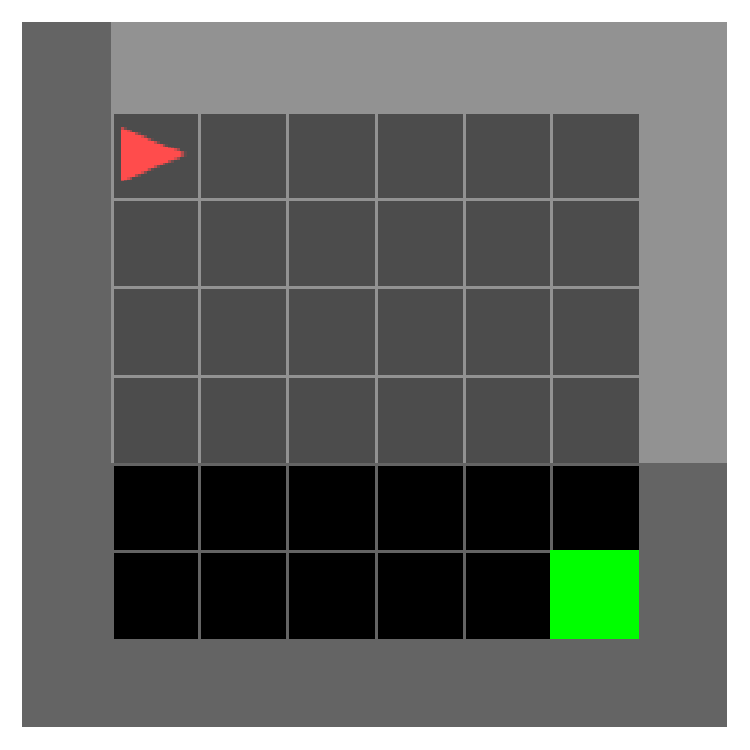
\includegraphics[width=0.9\linewidth]{figures/grid_world.pdf}
	\caption{The \texttt{MiniGrid-Empty-8x8-v0} environment}
	\label{fig:mini-grid}
\end{figure}

Depending on our configuration, the state can be a tensors, or an image which is returned after each actions. The agent have in total eight possible actions, but we only use three: turn left and right, and move forward. By this setting, we deal with an episodic task, and for each episode the agent can perform at most 256 steps.

If the agent reach the target, it receive a reward $r$ defined by:
\begin{equation}
	r = 1 - 0.9\times \frac{\text{Number of steps}}{\text{Maximum number of steps}}
\end{equation}
otherwise the reward is zero.


Therefore our task is to make the agent learns how to move in these grid in such a way that it maximize its reward. For this particular environments the agent can get at most a reward of $0.9613$ with $11$ steps. But for this works we will consider $0.9578$ as optimal reward corresponding to 12 steps.

\section{Reinforcement Learning technique}
In this era, reinforcement learning is widely used to solve the problem of programming intelligent agents that learn how optimise a specific task such as playing game, autonomous vehicle. This is done by learning a policies for sequential decision problems that maximize the discounted  cumulative future reward:
\begin{equation}
	G_t \bydef \sum_{k=t+1}^{T} \gamma^{k-t-1}R_k
\end{equation}
Where $R$ is the reward, $\gamma\in [0,1]$ the discount factor that control the importance fro immediate reward (near to 0) or future reward (near to 1). The agent learn the optimal policy without being explicitly told if its action are good or bad using the reinforcement learning model depicted in the Figure \ref{fig:RL}.


\begin{figure}
	\centering
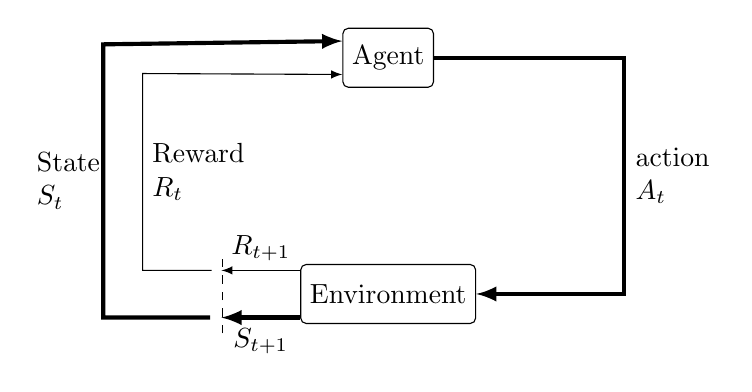
\begin{tikzpicture}
\node[draw, rounded corners=2pt, minimum height=.75cm] (agent) at (0,0) {Agent};
\node[draw, rounded corners=2pt, minimum height=.75cm] (env) at (0,-3) {Environment};
\draw[->, >=latex,line width=1.5pt] (agent) -- (3, 0) -- node[right,midway, text width=1cm] {action\\$A_t$} (3, -3) -- (env);
\draw[->, >=latex] (env.165) --node[above] {$R_{t+1}$} ++(-1, 0) node (r) {};
\draw[->, >=latex, line width=1.5pt] (env.195) --node[below] {$S_{t+1}$} ++(-1, 0) node (s) {};
\draw[->, >=latex] (r) -- ++(-1, 0) --node[right, midway, text width=1cm] {Reward\\$R_t$} ++(0, 2.5)-- (agent.200);
\draw[->, >=latex,line width=1.5pt] (s)-- ++(-1.5, 0) --node[left=-0.3cm, midway, text width=1cm] {State\\$S_t$} ++(0, 3.47) -- (agent.160);
\draw[dashed] (-2.1, -3.5)--(-2.1, -2.5);
\end{tikzpicture}
\caption{Reinforcement learning Model}
\label{fig:RL}
\end{figure}

Several algorithms/technique can be used  to solve our problem with reinforcement leaning, in the next section we will look:
\begin{itemize}
	\item Q-Learning
	\item SARSA (State-Action-Reward-State-Action)
	\item Deep Q-Network
	\item Deep Q-Network with RGB Image techniques.
\end{itemize}
The algorithm \ref{algo:rl_skel} show the skeleton shared by these RL algorithm.
\begin{algorithm}
Parameters:$\ldots$\\
\ForEach{episode}{
	(Re)Initialize the environment\\
\ForEach{step}{
Perform an action and consider the obsrvation and reward\\
\textbf{Steps specific to each methods}\\
\If{done or truncated}{
Some step for metric and monitoring\\
}
}
}
\caption{RL Algorithm Skeleton}
\label{algo:rl_skel}
\end{algorithm}
In addition to that, we also use the $\epsilon$-greedy strategy to select the action to be performed by the agent. The agent uniformly sample an action from the possible action for the given state with a probability $\epsilon$, and use the optimal action for the given state with a probability $1-\epsilon$. In the first case we say that the agent is exploring, and it the second case we say that the agent is exploiting.


For this works we will start with a higher value of $\epsilon$ to allow to the agent to explore all the environment, then we decrease it slowly until we reach a small value, this will be controlled by :
\begin{equation}
\epsilon_t = \epsilon_{min} + \left(\epsilon_{max} - \epsilon_{min}\right) \exp\left\{-\frac{t}{\Delta}\right\}
\end{equation}
Where $\Delta$ is the decay rate, a higher value correspond to a slow decrease, and a small value correspond to fast decrease.
\section{Tabular methods: Q-Learning and SARSA}
Tabular method, refer to a creation of a table called Q-table, containing the value of $Q(S_t=s,A_t=a)$. This value indicate how good is performing the action $a$ on the state $s$.

For the two algorithm that we present in this section, the observation (a $7\times3\times3$ array) will be converted into a string to create a MD5 hash to represent the given state.
\subsection{SARSA}
The SARSA algorithm is an on-policy methods, that means it iteratively refine a single policy, that also generates controls action within the environments. The update rule is defined by:
\begin{equation}\label{eq:sarsa}
	Q(S_t, A_t)\leftarrow Q(S_t, A_t) + \alpha[R_{t+1} + \gamma(S_{t+1}, A_{t+1}) - Q(S_t, A_t)]
\end{equation}
Form the equation \eqref{eq:sarsa}, we obtain the Algorithm \ref{algo:sarsa} fo the SARSA learning.
\begin{algorithm}
	Parameters: Step size $\alpha\in]0,1]$, small $\epsilon>0$\\
	Initialize $Q(s,a)$ for all $s\in\mathcal{S}^{+}$ and $a\in\mathcal{A}(s)$ arbitrarily, except that $Q(terminal-state, \cdot)=0$\\
	\ForEach{episode}{
		Initialize $S$\\
		Choose $A$ from $S$ using policy derived from $Q$ ($\epsilon$-greedy)\\
		\ForEach{step until $S$ is a terminal  state}{
			Take the action $A$, observe $R$, $S'$\\
			Choose $A'$ from $S'$ using policy derived from $Q$ ($\epsilon$-greedy)\\
			$Q(S, A)\leftarrow Q(S, A)$\\
			\phantom{$Q(S, A)\leftarrow$}$ + \alpha[R_{t+1} + \gamma(S', A') - Q(S_t, A_t)]$\\
			$S\leftarrow S'$\\
			$A\leftarrow A'$
		}
	}
\caption{SARSA: on-policy learners to estimate the optimal Q-table}
\label{algo:sarsa}
\end{algorithm}

\subsection{Q-Learning}
In contrast of SARSA, the $Q$-Learning algorithm is an off-policy algorithm, that mean we optimise the target policy using different policy. The update rule is given by
\begin{equation}\label{eq:qlr}
	Q(S_t, A_t)\leftarrow Q(S_t, A_t) + \alpha[R_{t+1} + \gamma\max_a (S_{t+1}, a) - Q(S_t, A_t)]
\end{equation}
Since, we have the Algorithm \ref{algo:qlr} for $Q$-learning methods.
\begin{algorithm}
	Parameters: Step size $\alpha\in(0,1]$, small $\epsilon>0$\\
	Initialize $Q(s,a)$ for all $s\in\mathcal{S}^{+}$ and $a\in\mathcal{A}(s)$ arbitrarily, except that $Q(terminal-state, \cdot)=0$\\
	\ForEach{episode}{
		Initialize $S$\\
		Choose $A$ from $S$ using $\epsilon$-greedy\\
		\ForEach{step until $S$ is a terminal  state}{
			Take the action $A$, observe $R$, $S'$\\
			Choose $A'$ from $S'$ using $\epsilon$-greedy\\
			$Q(S_t, A_t)\leftarrow Q(S_t, A_t) + \alpha[R_{t+1} + \gamma\max_a (S_{t+1}, a) - Q(S_t, A_t)]$\\
			$S\leftarrow S'$\\
		}
	}
	\caption{Q-learning algorithm to estimate the optimal $Q$-table}
	\label{algo:qlr}
\end{algorithm}



These two methods are powerful to deal with few states and action, but not very efficient to deal with a high number of states and action. We can replace the table by a function approximator as we will see in the next section.



\section{Function approximation: Deep $Q$-network}
The idea of function approximation is to replace the value function by its approximation instead of using a look-up table. The function can take
\begin{itemize}
	\item the state and action as input, and $q(s,a)$ as output,
	\item or the state as input and $q(s,a)$ as output.
\end{itemize}
This is illustrated in the figure \ref{fig:fct-approx}.
\begin{figure}
	\centering
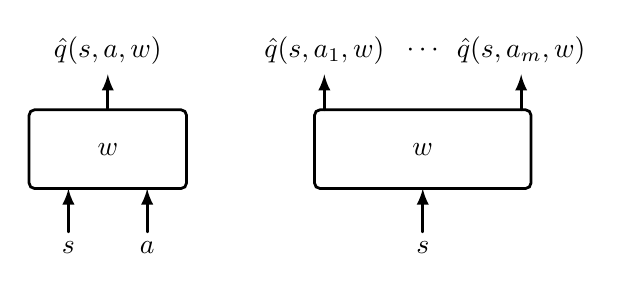
\begin{tikzpicture}
\begin{scope}
		\node (s) at (-0.5,-1.25) {$s$};
	\node (a) at (0.5,-1.25) {$a$};
		\node (q) at (0,1.25) {$\hat{q}(s, a, \mbf{w})$};
	\node[draw, rounded corners=2pt, line width=1pt, minimum width=2cm, minimum height=1cm] (fct) at (0,0) {$\mbf{w}$};
	\draw[->, >=latex,line width=1pt, line cap=round] (s) --++(0,0.75);
	\draw[->, >=latex,line width=1pt, line cap=round] (a) --++(0,0.75);
	\draw[->, >=latex,line width=1pt, line cap=round] (fct) -- (q);
\end{scope}
\begin{scope}[xshift=4cm]
	\node (s) at (0,-1.25) {$s$};
	\node (q1) at (-1.25,1.25) {$\hat{q}(s, a_1, \mbf{w})$};
	\node (q2) at (0,1.25) {$\cdots$};
	\node (q3) at (1.25,1.25) {$\hat{q}(s, a_m, \mbf{w})$};
	\node[draw, rounded corners=2pt, line width=1pt, minimum width=2.75cm, minimum height=1cm] (fct) at (0,0) {$\mbf{w}$};
	\draw[->, >=latex,line width=1pt, line cap=round] (s) --++(0,0.75);
	\draw[<-, >=latex,line width=1pt, line cap=round] (q1) --++ (0, -.75);
	\draw[<-, >=latex,line width=1pt, line cap=round] (q3) --++ (0, -.75);
\end{scope}
\end{tikzpicture}
\caption{Illustration of function approximation}
\label{fig:fct-approx}
\end{figure}


In our case, we will use neural network as function approximation. Thus we will consider two types.

A feed forward neural network (MLP) which take a vector $\mbf{u}\in\RR^{49\times1}$ (state) as input and $q(s,a_1), q(s,a_2),q(s,a_3)$ as output.

Similarly, a Convolutional Neural networks (CNN), which take a stack of four frames (images) at four successive time steps, e.g. a $4\times56\times56$ tensor as input and same output as the MLP,. The architecture of these neural networks are described in respectively in REF-MLP and REF-CNN.


As we do not have any labels to train the networks, we use two networks: the \texttt{policy\_net} and \texttt{target\_net}. The first one is optimised with the \texttt{Adam} optimizer, while the second one is fixed, and used to generate a sort of label for the \texttt{policy\_net}. We also synchronize the weight of the two network in aregular period of the training, to move toward into the optimal values.


To train these networks, we need a dequeue (double end-queue) that store a given number of the experience of the agent formed by the current state, action, next state, and reward, we call this a replay memory $\mathcal{D}$. As new experience are added the oldest data is pushed out of the dequeue.
Once we reach have batch size (enough number) of experience, we start to sample from $\mathcal{D}$ and optimize the \text{policy\_net} parameter by minimizing the Mean Squared Error (MSE) given by:
\begin{equation}
	\mathcal{L} = \frac{1}{N}\sum{i=1}^{N}\left[R_i + \gamma\max_{a'}\hat{Q}(s_i', a', \mbf{w}^{-}) - \hat{Q}(s_i, a, \mbf{w})\right]^2
\end{equation}
where $R_i + \gamma\max_{a'}\hat{Q}(s_i', a', \mbf{w}^{-})$ is computed using \texttt{target\_net}, and $\hat{Q}(s_i', a', \mbf{w}^{-})$ is $0$ if $s_i'$ is terminal state, while $\hat{Q}(s_i, a, \mbf{w})$ is computed with \texttt{policy\_net}.


Note that, the input of these network (observation) are normalized by rescaling their value between $[-1,1]$, particularly we convert the RGB image into agrey-scale image for the CNN architecture.
We can summarize the whole process in the algorithm \ref{algo:dqn}.
\begin{algorithm}
	Initialize \texttt{policy\_net} and \texttt{target\_net}\\
	Initialize the environments\\
	Set the decay rate for the epsilon decreasing\\
	Set the updating period of \texttt{target\_net}\\
	Set the total step to $0$\\
	Create a replay memory $\mathcal{D}$\\
	\ForEach{episode}{
	Set step to 0\\
	Make new episode\\
	Observe the first state\\
	\While{not( done or truncated)}{
	Choose $A$ from $S$ using policy derived from $Q$ ($\epsilon$-greedy)\\
	Increment the total training step\\
	Execute $A$, observe $R$ and the new state $S'$\\
	Store Transition $<S, A, S', R>$ in $\mathcal{D}$\\
	Compute the $\mathcal{L}$ and do a gradient descent step\\
	\If{updating period}{
	Copy the \texttt{policy\_net} parameter to \texttt{target\_net}
	}
	}
	}
	\caption{Training a DQN to estimate the optimal policy}
	\label{algo:dqn}
\end{algorithm}
\section{Hyper-parameters tuning and Evaluation}
\subsection{Hyper-parameters}
like all machine learning problem we have several parameter to tune to get the optima results. Grid search is one of the best methods, it iterate though all the possible combination of predefined parameters set. The drawback of this method is the time complexity which can explode considerably when we hyper-parameter space is big and the algorithm is quite slow.

So, instead of using that approach we will use a intelligent trial an error to find the good hyper-parameter such as $\gamma$, $\alpha$, and the number of episodes. To do that we start we some values, and we adjust these parameter according to the obtained results.

\subsection{Model evaluation}
To evaluate the model, we run the the agents in the environment for $1000$ episodes, then compute the completion rate, the reward average, and the averaged steps for each methods.

We also investigate these value for the training process to asses the speed and efficiency of each methods, in addition of the plot of the loss and accumulated rewards.
\section{Results and discussion}
\section{Conclusion}
%\begin{thebibliography}{1}
%\end{thebibliography}